\documentclass[10pt,a4paper]{amsart}
\usepackage[margin=19mm]{geometry}
\usepackage{amsmath,amssymb,mathtools}
\usepackage[scr=rsfs,cal=euler]{mathalfa}
\usepackage{xfrac}
\usepackage[unicode,hidelinks,bookmarks=false]{hyperref}
\newcommand{\ie}{i.e.\ }
\newcommand{\cf}{cf.\ }
\newcommand{\resp}{respectively\ }
\newcommand{\Subsection}{\subsection}
\providecommand{\nobreakdash}{\nobreak\hbox{-}}
\setlength{\emergencystretch}{2em}
\multlinegap0pt
\usepackage{tikz}
\usepackage{amssymb}
\usepackage{bm}
\usepackage{mathtools}
\usepackage{xcolor}
\usepackage[shortlabels]{enumitem}
\newtheorem{lemma}{Lemma}
\newcommand{\C}{\mathcal C}
\title{Geometric Categories and Sheaves on Topoi}
\author{Connor Bass}
\date{Source: arXiv:2605.02115v1 (CC BY 4.0)}
\begin{document}
\maketitle

\noindent\emph{Source and licence.} Geometric Categories and Sheaves on Topoi. Version arXiv:2605.02115v1 (CC BY 4.0), distributed by arXiv under the Creative Commons Attribution 4.0 International licence, http://creativecommons.org/licenses/by/4.0/, as recorded in the arXiv licence metadata for this exact version and shown on the abstract page https://arxiv.org/abs/2605.02115v1. Full licence notice: \texttt{licenses/arxiv-2605.02115-CC-BY-4.0.txt}.\par\smallskip

\noindent\textit{Editorial scope.} Counted unit: the article's lemma Slices (source0.tex lines 1888--1892). The article's complete original proof of it is delivered with it (source0.tex lines 1895--1916, one \texttt{proof} environment of 22 lines). No mathematics is written, repaired or re-derived: the statement and the proof are the article's own lines, in the article's own notation, and no retained line is substituted or re-flowed.  No further source-local context is needed: every cross-reference of every retained line resolves inside the two delivered spans.  Nothing was omitted from any retained span, so the package carries no omission record.  No retained line contains a citation, so the wrapper carries no bibliography and no bibliography entry.  The retained lines contain the article's own diagram code, which the wrapper typesets with the standard tikz packages; no image file is delivered and the package declares no asset dependency.  Editorial formatting only, in addition: an AMS \texttt{amsart} preamble that restates the article's own declarations and macros used by the retained lines, namely the environments \texttt{lemma} on separate counters, together with the standard packages those lines need.  The retained environments print in this document as Lemma 1 in order of appearance, whereas the article prints the same items with the numbering of its own full document.  The complete native source of the article as distributed in the arXiv e-print for this exact version is bundled unchanged as \texttt{sources/199695/source0.tex}.
\begin{lemma}{}\label{Reflective Localizations and Slices}

    Let $\C$ be an $(\infty,1)$-category, let $S$ be a collection of arrows in $\C$, and let $\C^\prime\subseteq \C$ be the full subcategory spanned by the $S$-local objects. Let $X\in \C^\prime$, and write $p:\C_{/X}\rightarrow \C$ for the projection. Then, $\C^\prime_{/X}\subseteq \C_{/X}$ may be identified as the full subcategory spanned by the $p^{-1}(S)$-local objects. 

\end{lemma}

\begin{proof}

    Let $h:U\rightarrow X$ be an object in $\C_{/X}$, which we will denote by $\overline{U}$. Let $f:A\rightarrow B$ be a map in $S$. Consider the homotopy commuting square 

    $$
            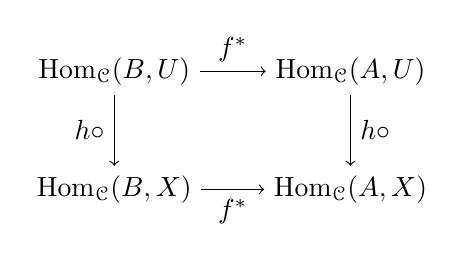
\begin{tikzpicture}[node distance=1.5cm, auto]
                \node (A) {$ \textnormal{Hom}_\C(B,U)
                $};
                \node (A1) [right of=A] {$ $};
                \node (B) [right of=A1] {$ \textnormal{Hom}_\C(A,U)$};
                \node (C) [below of=A] {$ \textnormal{Hom}_\C(B,X) $};
                \node (D) [below of=B] {$  \textnormal{Hom}_\C(A,X) $};
                \draw[->] (A) to node {$ f^* $} (B);
                \draw[->] (A) to node [swap] {$ h\circ $} (C);
                \draw[->] (C) to node [swap] {$ f^* $} (D);
                \draw[->] (B) to node {$ h\circ $} (D);
            \end{tikzpicture}
    $$

    \noindent This is a homotopy pullback square if and only if, for each $g:B\rightarrow U$ in $\C$, the induced map on homotopy fibres $\textnormal{Hom}_\C(B,U)_{g}\rightarrow \textnormal{Hom}_\C(A,U)_{g\circ f}$ is a homotopy equivalence. Since the bottom arrow is a homotopy equivalence (as $f\in S$ and $X\in \C^\prime$), this implies that $f^*:\textnormal{Hom}_\C(B,U)\rightarrow \textnormal{Hom}_\C(A,U)$ is a homotopy equivalence if and only if each $\textnormal{Hom}_\C(B,U)_{g}\rightarrow \textnormal{Hom}_\C(A,U)_{g\circ f}$ is a homotopy equivalence. Placing $B$ over $X$ via $h\circ g:B\rightarrow X$ (call this $\overline{B}\in \C_{/X}$), and placing $A$ over $X$ via $h\circ g\circ f:A\rightarrow X$ (call this $\overline{A}\in \C_{/X}$), we see that the induced map $\textnormal{Hom}_\C(B,U)_{g}\rightarrow \textnormal{Hom}_\C(A,U)_{g\circ f}$ may be identified as the arrow $\textnormal{Hom}_{\C_{/X}}(\overline{B},\overline{U})\rightarrow \textnormal{Hom}_{\C_{/X}}(\overline{A},\overline{U})$ given by pulling-back along the obvious arrow $\overline{f}:\overline{A}\rightarrow \overline{B}$ satisfying $p(\overline{f})=f$.  Thus, $\overline{U}\in \C_{/X}$ is local with respect to $p^{-1}(S)$ precisely when $U\in \C$ is local with respect to $S$.
    
\end{proof}

\end{document}
